\documentclass[slovene,11pt,a4paper]{article}
\usepackage[margin=1.8cm,bottom=3cm,foot=1.5cm]{geometry}
\usepackage{amsmath}
\usepackage{booktabs}
\usepackage{float}
\usepackage{graphicx}
\usepackage{gensymb}
\usepackage{geometry}
\usepackage{changepage}
\usepackage{subcaption}
\usepackage{multirow}
\usepackage{blindtext}
\usepackage{hyperref}
\usepackage[version=4]{mhchem}
\usepackage[slovene]{babel}
\pagenumbering{gobble}
\renewcommand{\contentsname}{\centering Contents}

\begin{document}

\title{8. naloga - Metropolisov algoritem}
\author{Tadej Lozej 28201055}
\maketitle
\begin{center}
Modelska analiza 1 \\
\bigskip
Predavatelj: prof. dr. Simon Širca \\
Asistent: doc. dr. Miha Mihovilovič
\end{center}

\newpage

\tableofcontents

\newpage

\section{Uvod}

\pagenumbering{arabic}

Metropolisov algoritem je algoritem s katerim si lahko pomagamo pri iskanju energijskih minimumov različnih sistemov. Algoritem temelji na naključnem preurejanju našega sistema. Če je nova ureditev energijsko ugodnejša jo obdržimo, če ni energijsko ugodnejša pa jo obdržimo le z določeno verjentostjo. Recimo, da je naš sistem ob nekem času $t$ v stanju $X_t$. Nato izžrebamo neko novo stanje sistema $Y_t$ in se odločimo ali je to stanje ustrezno za naslednje stanje $X_{t+1}$ ali ne kot

\begin{equation}
X_{t+1} = 
	\begin{cases}
	Y_t; \text{ z verjetnostjo } \text{min} \left(1, \frac{P(Y_t)}{P(X_t)} \right)\\
	X_t; \text{ sicer}
	\end{cases}
\end{equation}
kjer je $P(X_t) = e^{-E(X_t)/k_BT}$ in $P(Y_t) = e^{-E(Y_t)/k_BT}$. Po tej zanki nato delamo poteze. V nalogi si Metropolisov algoritem pogledamo na primeru Molekularne verižnice ter Isingovega modela.

\section{Molekularna verižnica}

Molekularna verižnica je v našem primeru sedemnajst členkov dolga nitkasta molekula je obešena za oba konca. Vsak členek se lahko povesi od ničelne lege na poljuben nivo in si s tem zmanjša potencialno energijo za eno enoto na nivo. Če pa s tem prenategne vezi do sosedov, plača s prožnostni energijo, ki je za vsakega soseda enaka kvadratu razlike v nivojskem številu. Energija verižnice je tako enaka

\begin{equation}
E = \sum_{i=1}^{17} \alpha h_i + \sum_{i=1}^{16} \frac{1}{2} (h_{i+1} - h_i)^2,
\end{equation}
kjer je $h_i$ nivo $i-tega$ členka.

Število nivojev na katere se lahko členki v verižnici postavijo omejimo na 19. Tako je $h_i$ lahko le celo število med 0 in -18. Nalogo rešujemo v programskem jeziku \texttt{Python}. Začnemo z naključno konfiguracijo členkov in izračunamo energijo te konfiguracije. En korak v našem algoritmu pomeni to, da naključno izberemo enega izmed členkov verižnice ter mu nivo spremenimo naključno za $+1$ ali $-1$. Izračunamo spremembo energije konfiguracije in se po enačbi (1) odločimo ali novo konfiguracijo obdržimo ali ne.

Na sliki 1 so prikazane konfiguracije verižnice pti različnih korakih za različne vrednostih $\alpha$ in $k_BT$. Prikazana je začetna naključna konfiguracija verižnice ter konfiguracija verižnice pri $200$, $400$, $600$ in $800$ korakih. Iz slike lahko sklepamo, da verižnica hitreje pride do ravnovesnega stanja pri nižjih vrednostih $k_BT$, saj ima manjšo možnost da sprejme konfiguracijo z večjo energijo. Sicer bi pri nizkih temperaturah lahko imeli problem z izhodom iz lokalnih minimumov a v teh primerih do tega ni prišlo. Na sliki vidimo tudi to, da večja kot je vrednost $\alpha$ nižje želijo členki verižnice, saj so njihove koordinate $h_i$ v enačbi (2) bolj otežene. Pri vrednosti $\alpha=10$ vidimo, da so v minimumu energije že skoraj vsi členki pri minimalno dovoljeni vrednosti $h_i = -18$, medtem ko pri vrednosti $\alpha=0.1$ ima najnižji členek po $500$ korakih vrednost $h_i = -14$.

Na sliki 2 si poglejmo še, kako se v odvisnosti od števila korakov spreminja energija, ter oba člena v vsoti energije povprečna višina členkov in povprečen kvadrat razlike višine med sosednjimi členki. Pri energiji v odvisnosti od števila korakov vidimo, da se vrednost ustali hitreje za manjše vrednosti $k_BT$. Na drugih dveh grafih pa vidimo kateri člen v enačbi (2) v odvisnosti od $\alpha$. Vidimo, da za večje $\alpha$ je povprečna višina členkov po 1000 korakih manjša, medtem ko je povprečen kvadrat razlike višine sosednjih členkov večji. Ter obratno za manjše vrednosti $\alpha$.

\newpage

\begin{figure}[h!]
\centering
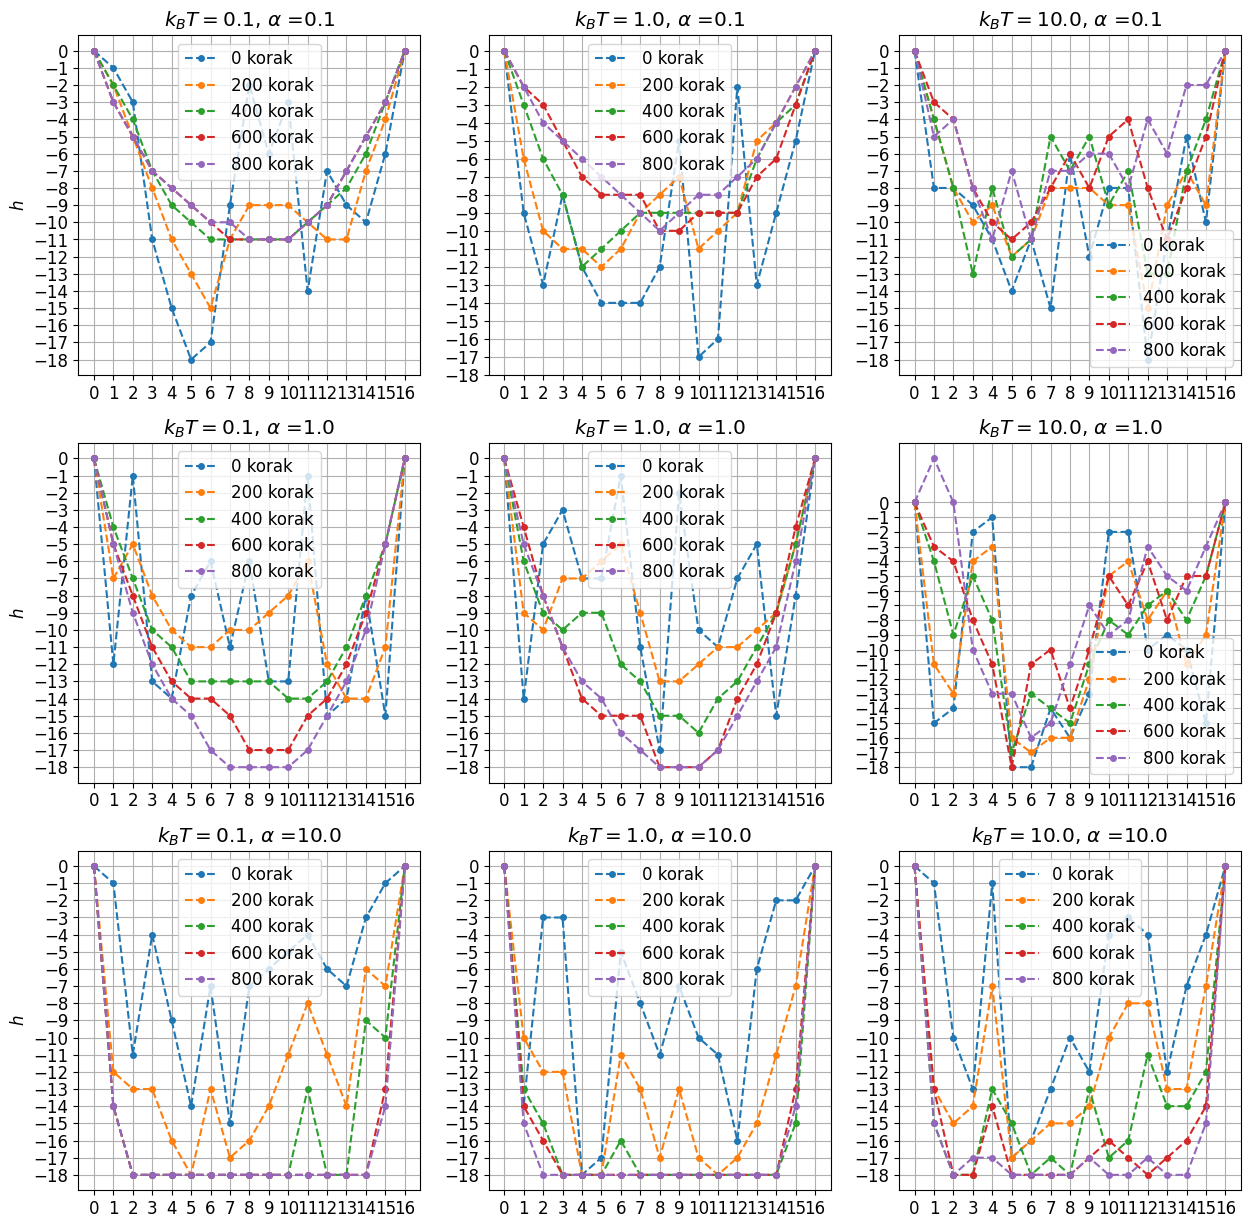
\includegraphics[width=\linewidth]{veriznica1.png}
\caption{Konfiguracija verižnice po številu korakov algoritma za več parov vrednosti $\alpha$ in $k_BT$. Sklepamo lahko, da za nižje temperature verižnica prej najde ravnovesno stanje. Prav tako vidimo, da za večje vrednosti $\alpha$ členki preferirajo nižje vrednosti $h_i$.}
\end{figure}

\newpage

\begin{figure}[h!]
\centering
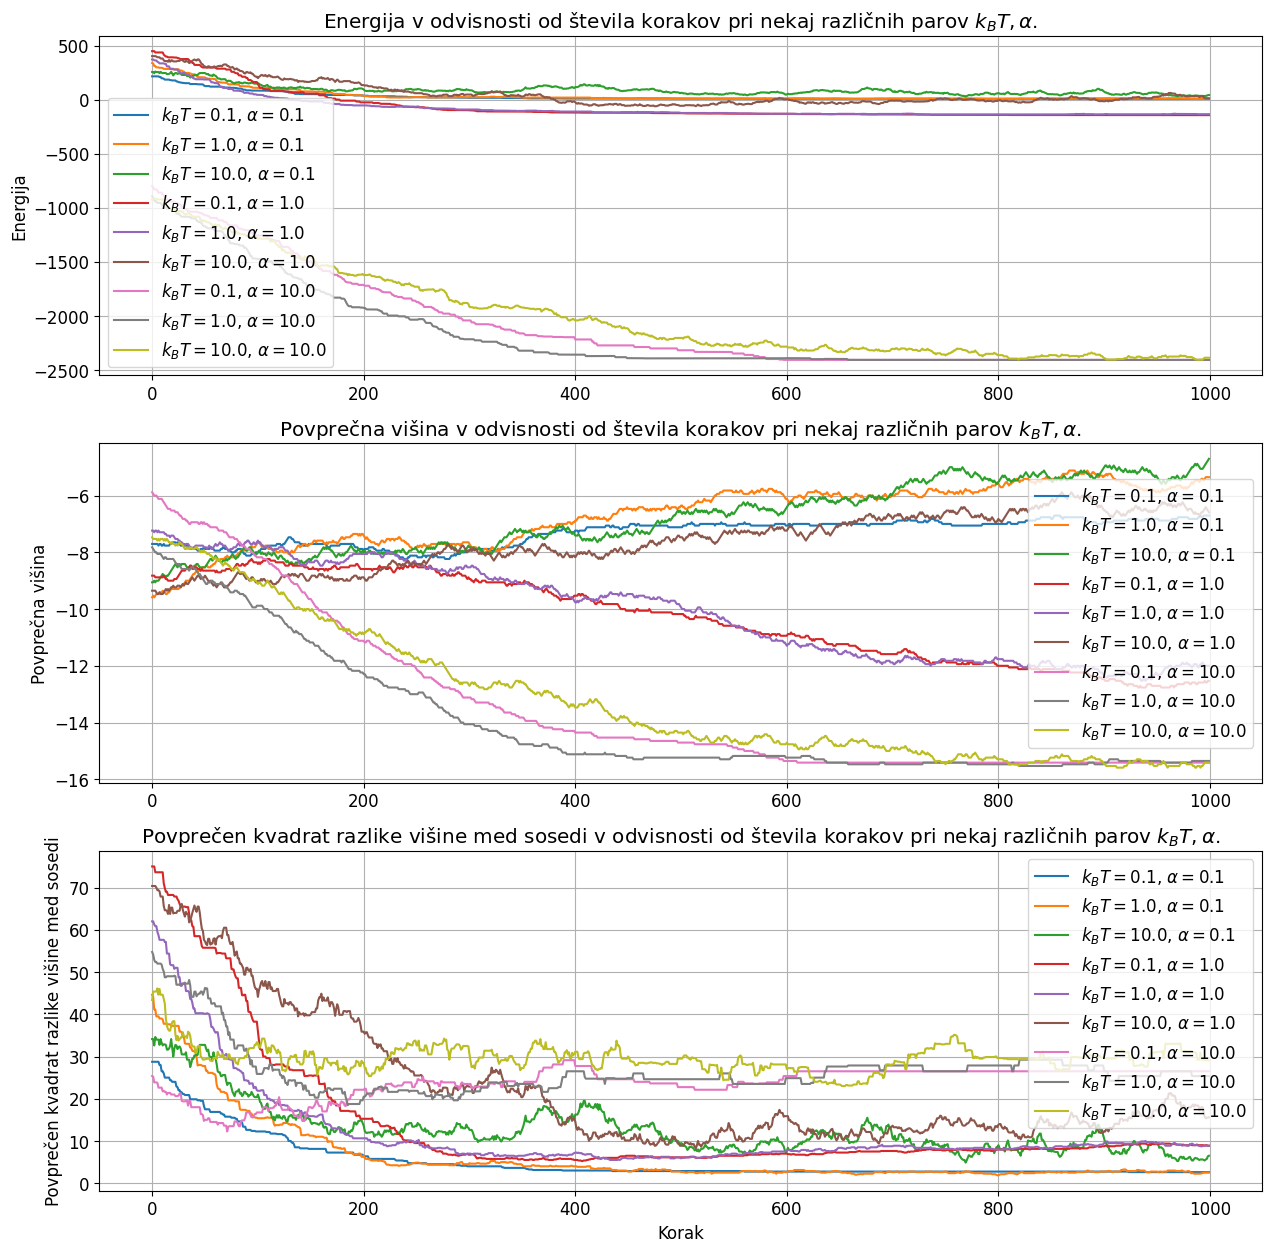
\includegraphics[width=\linewidth]{veriznica2.png}
\caption{Energije verižnice ter povprečna višina členkov in povprečen kvadrat razlike višine med sosednjimi členki v odvisnosti od števila korakov.}
\end{figure}

Na sliki 3 si nato lahko ogledamopovprečno energijo verižnice ter njeno varianco, ko se ta enkrat približno ustali, v odvisnosti od $k_BT$ za nekaj različnih $\alpha$. Prav tako je prikazana povprečna višina členkov ter povprečen kvadrat razlike višine sosednjih členkov v odvisnosti od $k_BT$ pri nekaj različnih vrednostih $\alpha$. Kot pričakovano energija povprečna energija v odvisnosti od $k_BT$ narašča, saj Sistem v resnici preživi največ časa v minimumu proste energije, ki je odvisna tudi od temperature in entropije. Tudi varianca energije se s temperaturo veča, saj je molekula bolj "živahna" pri višjih temperaturah. Za $\alpha$ kot pričakovano energija z večanjem vrednosti $\alpha$ pada. Vidimo, da tudi povprečna višina členkov in povprečen kvadrat oddaljenosti sosednjih členkov sta z večanjem $k_BT$ večja ter bolj raztresena.

\newpage

\begin{figure}[h!]
\centering
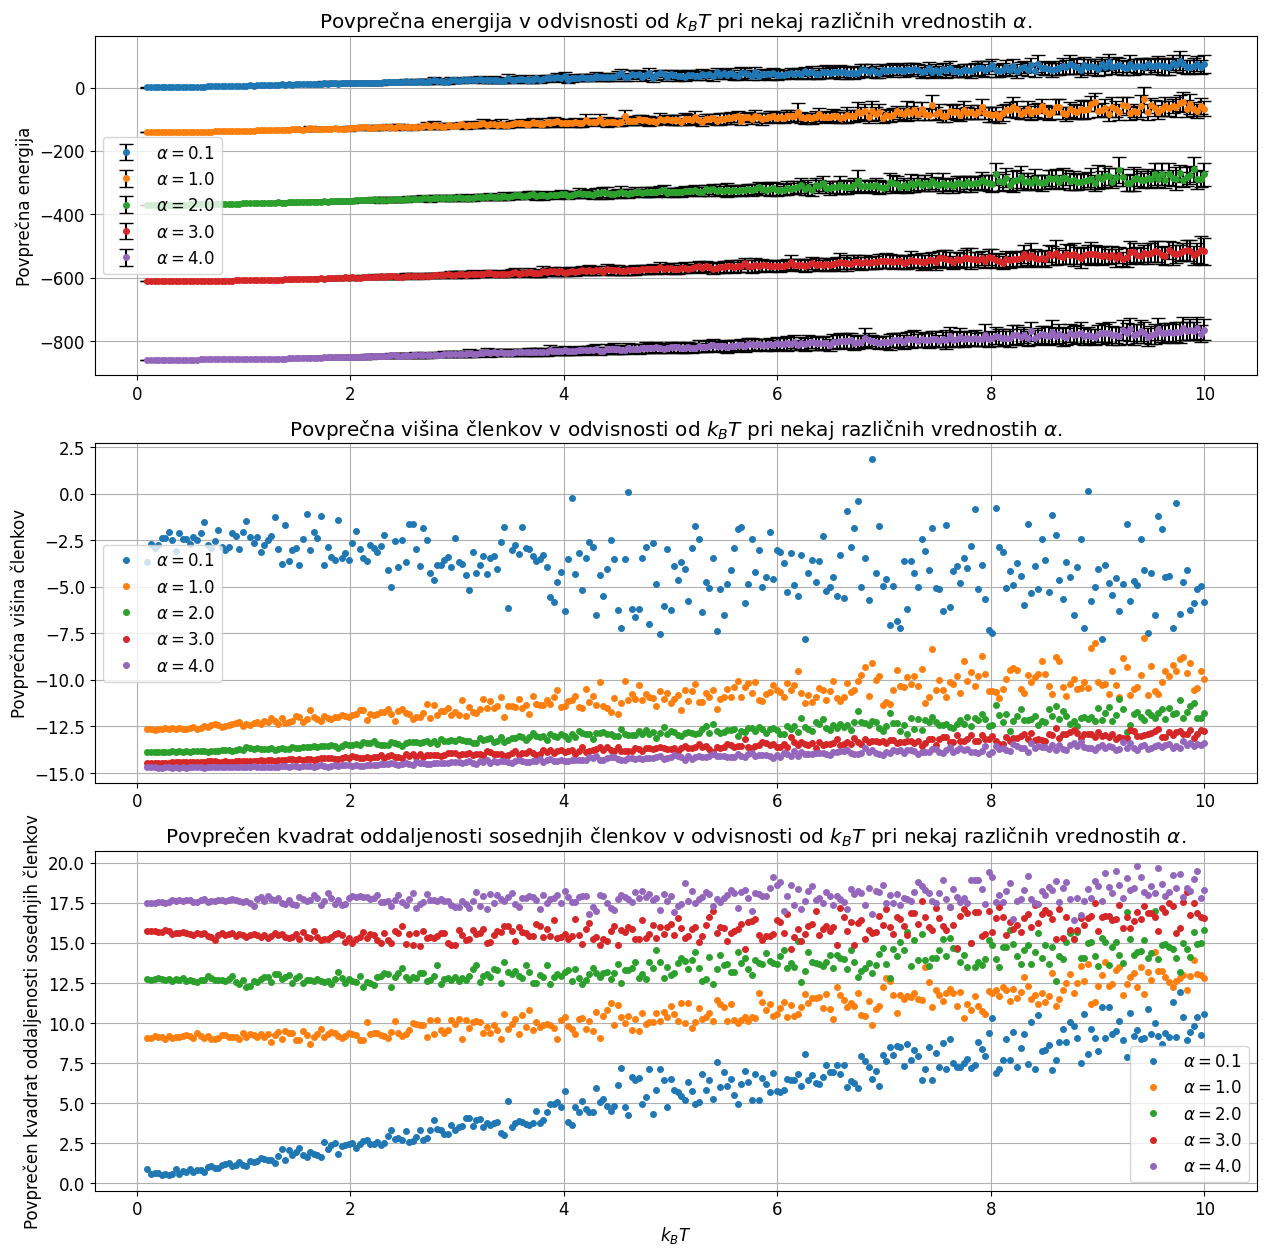
\includegraphics[width=\linewidth]{veriznica3.png}
\caption{Energije verižnice ter povprečna višina členkov in povprečen kvadrat razlike višine med sosednjimi členki v odvisnosti od števila korakov.}
\end{figure}

Na sliki 4 lahko vidimo še kako se verižnica oblikuje pri neomejeni vrednosti $h_i$ pri vrednostih parametrov $\alpha=0.1$ ter različnih vrednostih $k_BT$. Začnemo z naključnim stanjem v katerem imajo členki vrednosti $h_i$ med 0 in -10. Vidimo, da verižnica začne dobijati obliko verižnice.

\newpage

\begin{figure}[h!]
\centering
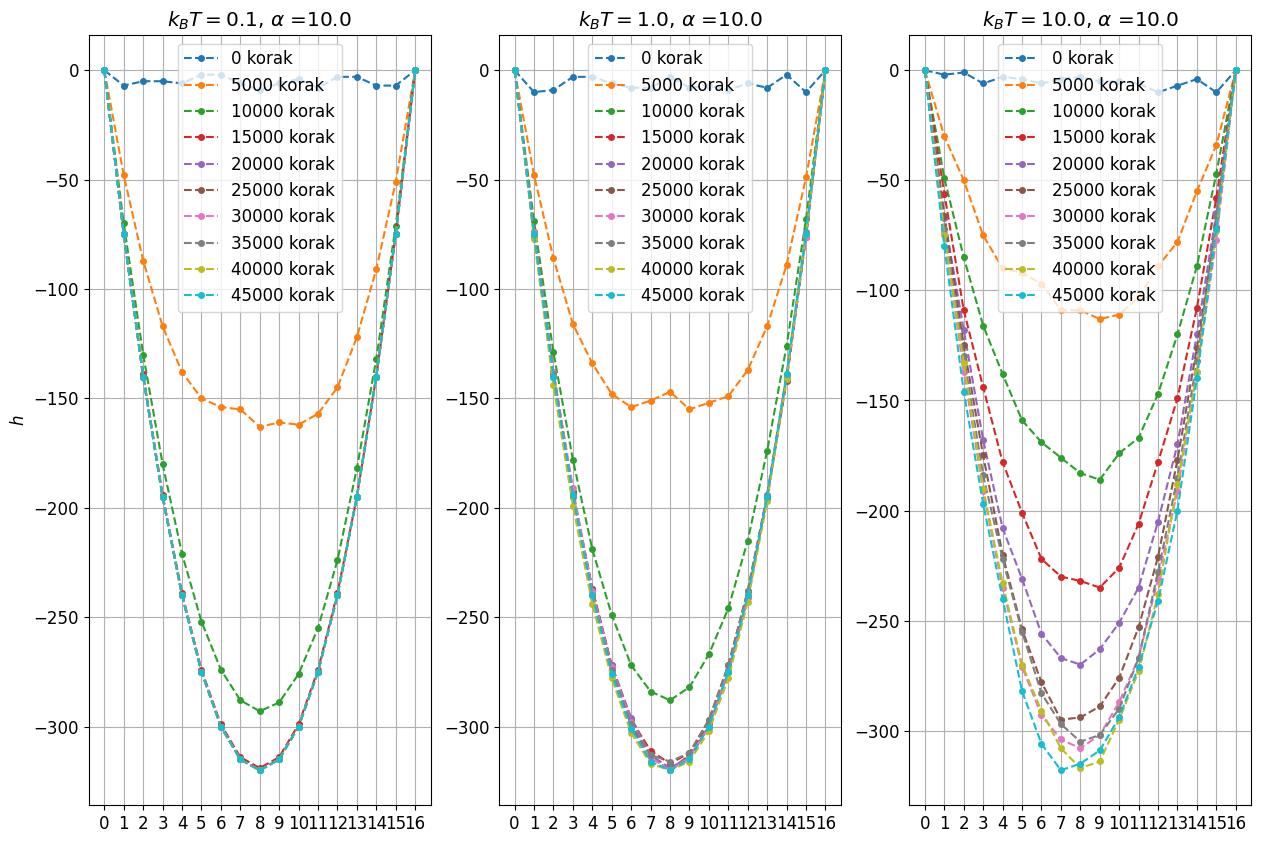
\includegraphics[width=\linewidth]{veriznica4.png}
\caption{Konfiguracija verižnice pri neomejeno vrednosti $h_i$. Vidimo, da verižnica dobi obliko verižnice.}
\end{figure}

\section{Isingov model}

Feromagnetne in antiferomagnetne snovi v dveh dimenzijah v približku dveh stanj opišemos Hamiltonovim operatorjem

\begin{equation}
\mathcal{H} = -J \sum_{\langle i,j \rangle} s_i s_j - H \sum_i s_i; \quad J = \pm 1,
\end{equation}
kjer je $s_i = \pm 1$ in vsota teče le po vezeh $\langle i,j \rangle$ med najbližjimi sosedi. K algoritmu pristopamo podobno kot v prvem poglavju. Izberemo naključno začetno konfiguracijo in ji izračunamo energijo po enačbi (3). Nato enega izmed spinov obrnemo in novo konfiguracijo obdržimo, če je ugodnejša oz. jo mogoče obdržimo, če ni ugodnejša.

\subsection{Ni magnetnega polja}

Če magnetnega polja ni temperatura $T_c$ faznega prehoda pšri feromagnetu zadošča enačbi

\begin{equation}
k_B T_c \approx 2.269185 \frac{J}{k_B}.
\end{equation}
Na sliki 5 je prikazana konfiguracija spinov za več vrednosti $k_BT$ pri različnih korakih algoritma. Upoštevamo periodični robni pogoj, saj se tako bolj približamo simulaciji neskončne snovi. Vidimo, da pri temperaturi nižji od temperature faznega prehoda se tvorijo očitne domene spinov v snovi, medtem ko pri večjih temperaturah se ne.

\newpage

\begin{figure}[h!]
\centering
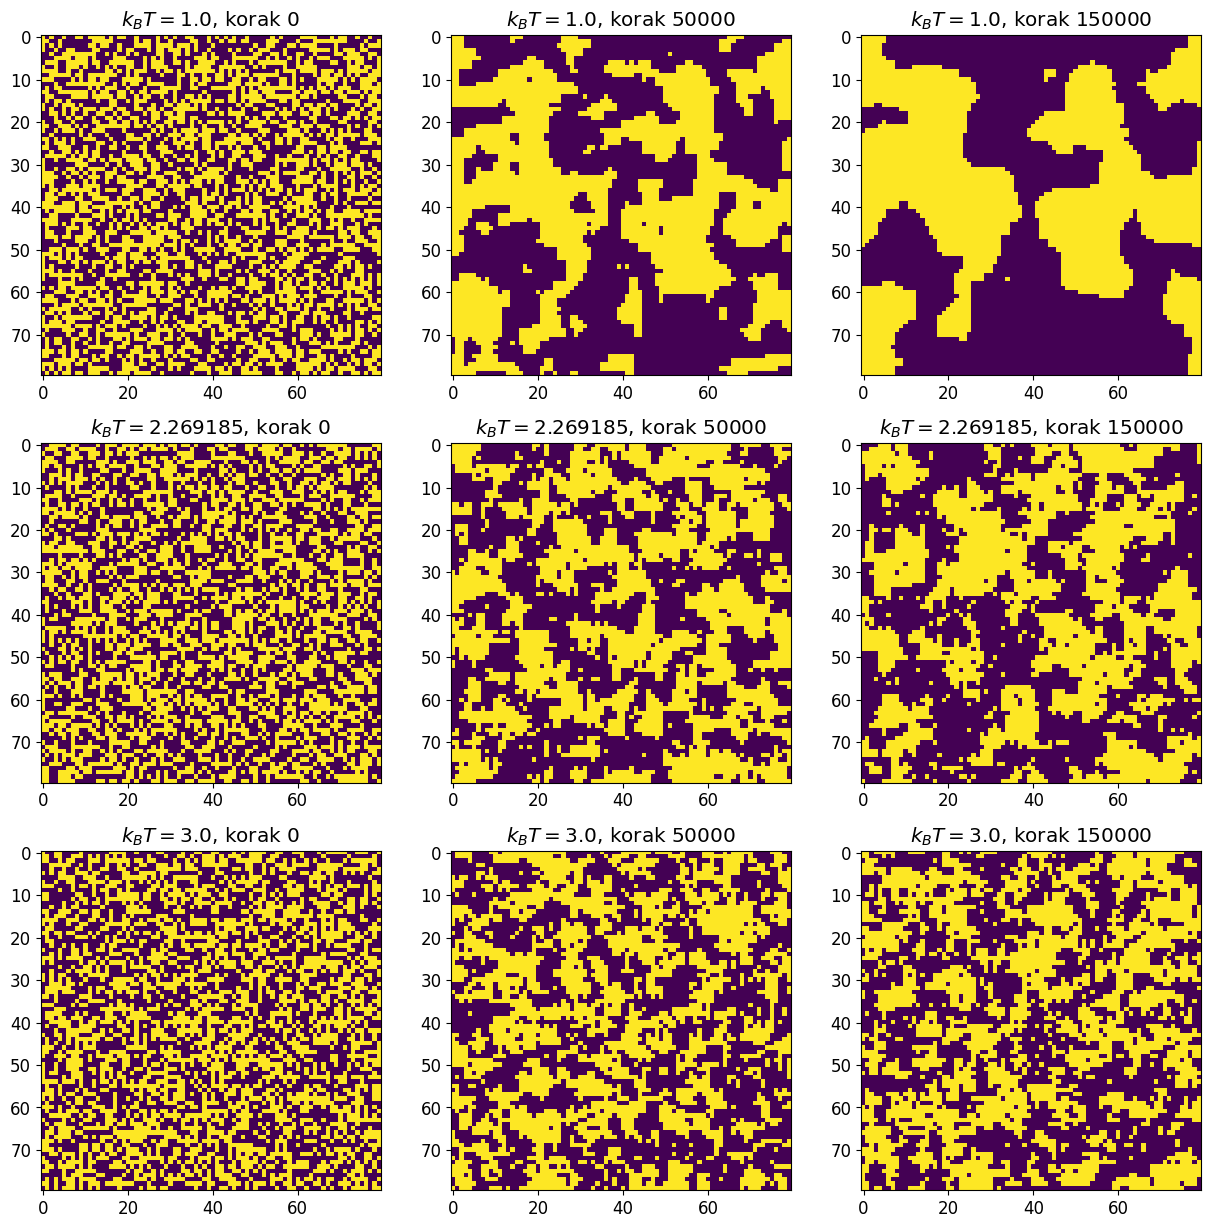
\includegraphics[width=\linewidth]{ising1.png}
\caption{Konfiguracija spinov v snovi pri različnih vrednostih $k_BT$ ustavljena pri več korakih.}
\end{figure}

Na sliki 6 je prikazana energija sistema v odvisnosti od števila korakov za nekaj različnih vrednosti $k_BT$. Vidimo, da za manjše $k_BT$ sistem doseže nižje energije kot za višje $k_BT$. Na sliki 7 je prikazano število domen v sistemu v odvisnosti od koraka. Prav tako vidimo, da je pri nižjih $k_BT$ število domen manjše kot pri višjih. Pomembno je dodati, da smo začeli z naključnim stanjem.

\newpage

\begin{figure}[h!]
\centering
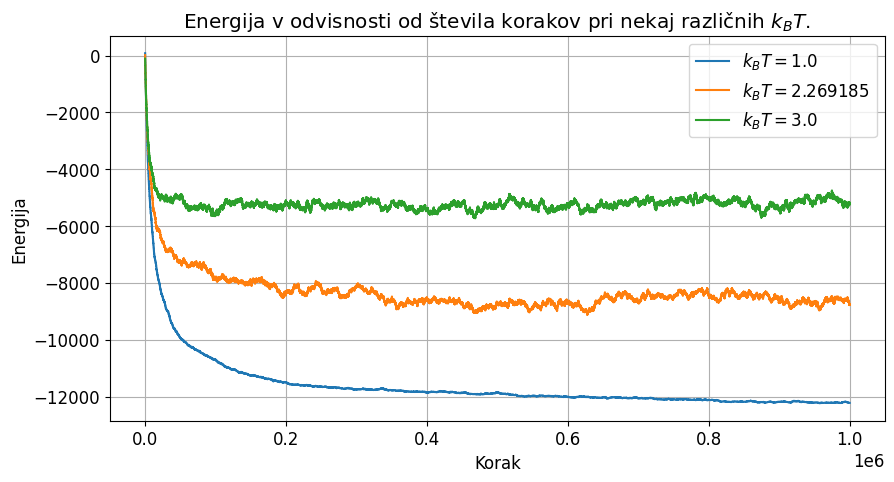
\includegraphics[width=\linewidth]{ising2.png}
\caption{Energija sistema v odvisnosti od števila korakov pri nekaj različnih vrednostih $k_BT$.}
\end{figure}

\begin{figure}[h!]
\centering
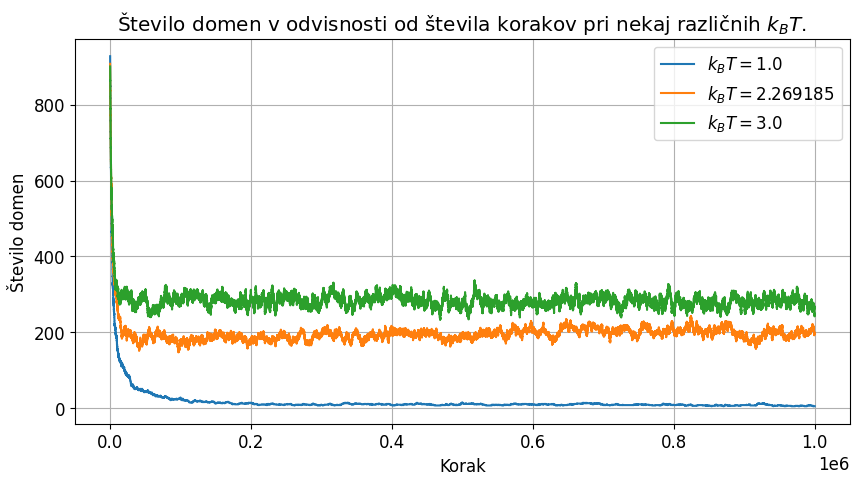
\includegraphics[width=\linewidth]{ising3.png}
\caption{Število domen v snovi v odvisnosti od števila korakov pri nekaj različnih vrednostih $k_BT$.}
\end{figure}

Magnetizacija je vsota po vseh spinih v konfiguraciji. Lahko jo izračunamo pri različnih $k_BT$. Prav tako lahko izračunamo tudi povprečno energijo in povprečno število domen pri različnih vrednostih $k_BT$. Vse to je prikazano na sliki 8. Za računanje povprečja in odstopanja sem vzel konfiguracije po 100000 korakih in začel sem že z delno urejenim stanjem.

\begin{figure}[h!]
\centering
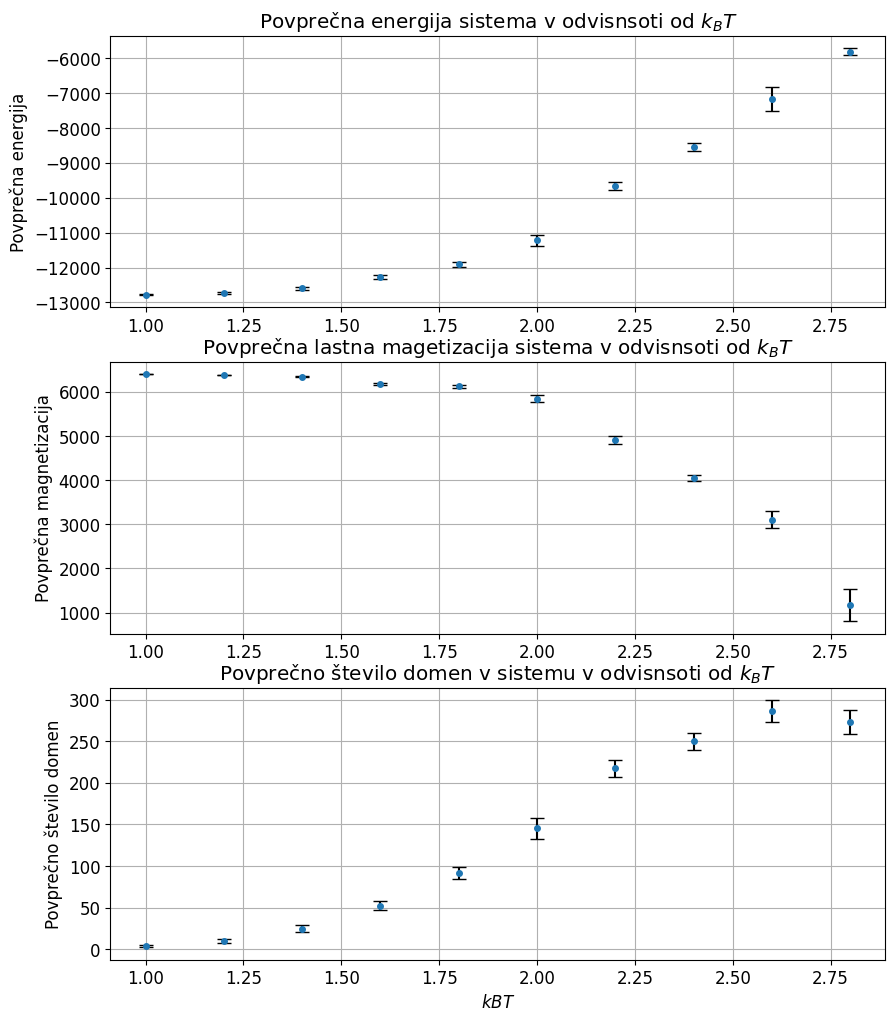
\includegraphics[width=\linewidth]{ising4.png}
\caption{Povprečna energija, povprečna lastna magnetizacija ter povprečno število domen v sistemu v odvisnosti od $k_BT$.}
\end{figure}

\subsection{Je magnetno polje}

V tem podpoglavju vključimo še magnetno polje. Poglejmo si povprečno energijo, povprečno lastno magnetizacijo in povprečno število domen v sistemu v odvisnosti od $k_BT$ pri nekaj različnih jakosti magnetnega polja. V tem poglavju bomo računali tudi susceptibilnost in specifično toploto. Slednji izračunamo po enačbah

\begin{equation}
\chi = \frac{\langle S^2 \rangle - \langle S \rangle^2}{Nk_BT}
\end{equation}
ter

\begin{equation}
\frac{c}{k_B} = \frac{\langle E^2 \rangle - \langle E \rangle^2}{Nk_B^2T^2}.
\end{equation}

Na sliki 9 sta prikazani susceptibilnost in specifična toplota sistema. Vidimo, da imata obe očiten vrh okrog neke temperature.

\begin{figure}[h!]
\centering
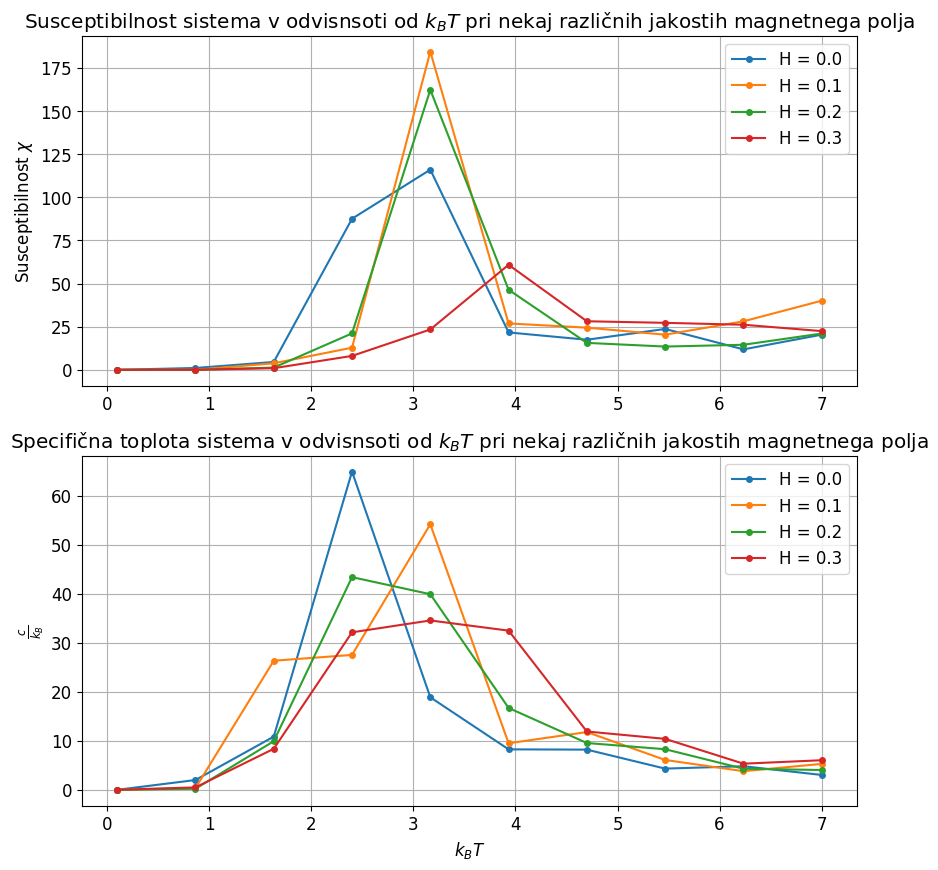
\includegraphics[width=\linewidth]{ising5.png}
\caption{Susceptibilnost in specifična toplota sistema v odvisnosti od $k_BT$ pri nekaj različnih vrednostih $H$.}
\end{figure}

Spodaj na sliki 10 pa vidimo povprečno energijo, povprečno lastno magnetizacijo in povprečno število domen v sistemu v odvisnosti od $k_BT$ pri nekaj različnih vrednostih $H$. Očiten vpliv magnetnega polja vidimo pri povprečni lastni magnetizaciji. Pri večjih $H$ je namreč lastna magnetizacija večja, saj spini preferirajo smer zunanjega magnetnega polja. Zanimiv je tudi vpliv velikosti gostote magnetnega polja na povprečno energijo sistema.

\begin{figure}[h!]
\centering
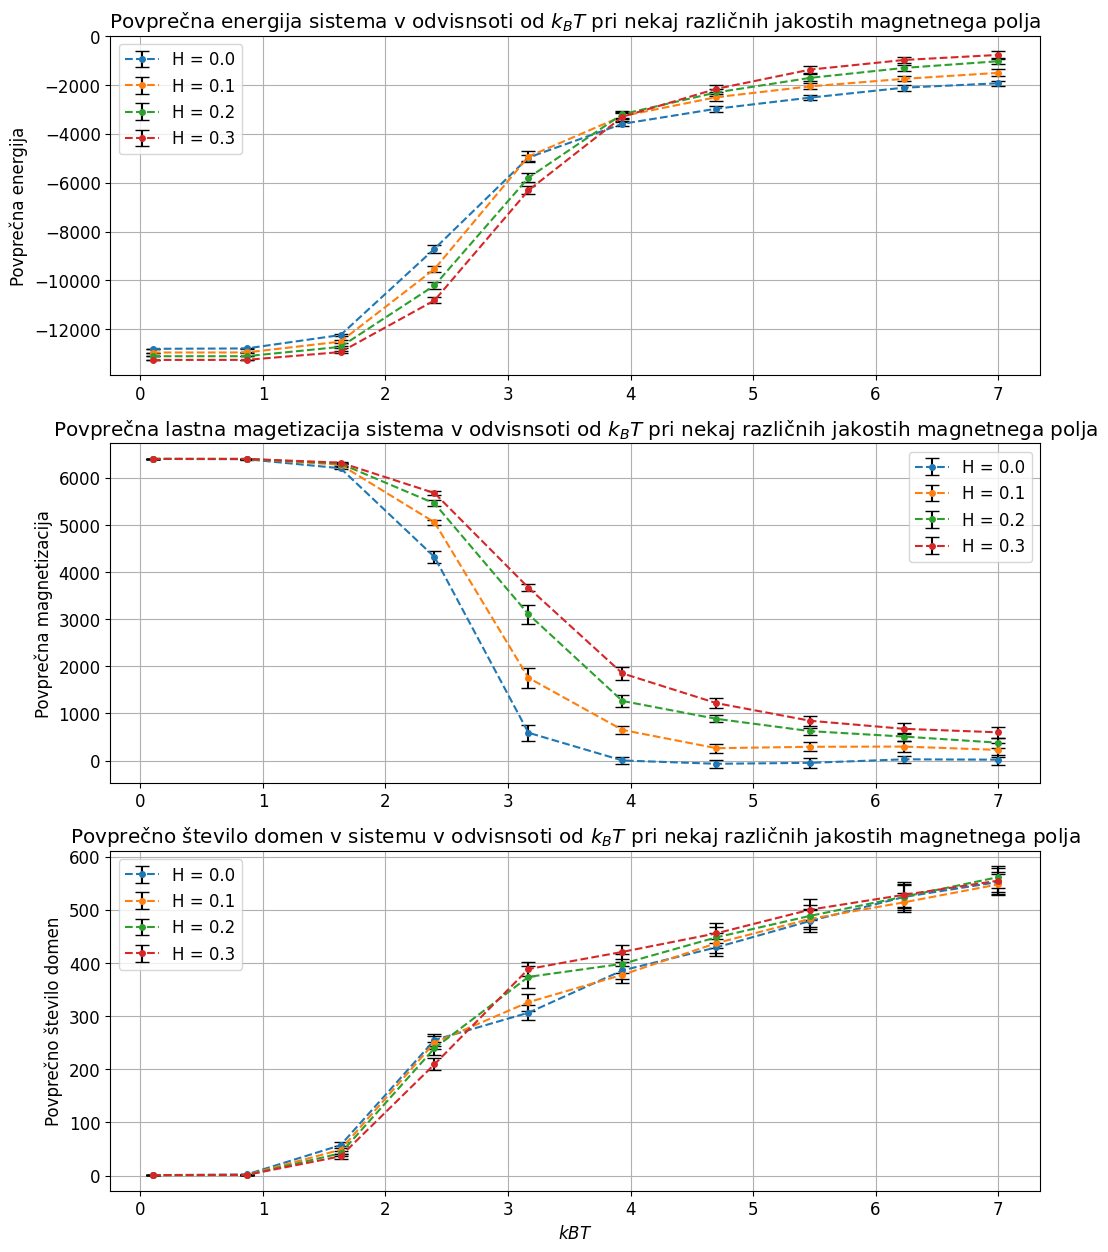
\includegraphics[width=\linewidth]{ising6.png}
\caption{Energija, povprečna lastna magnetizacija in povprečno število domen v sistemu v odvisnosti od $k_BT$ pri nekaj različnih vrednostih $H$.}
\end{figure}

Na sliki 11 je prikazano razmerje sprejetih potez v odvisnosti od $k_BT$ pri nekaj različnih vrednostih jakosti magnetnega polje $H$. Vidimo, da je razmerje sprejetih potez večje za višje vrednosti $k_BT$. Prav tako za manjša magnetna polja sprejmemo več potez kot za večja.

\newpage

\begin{figure}[h!]
\centering
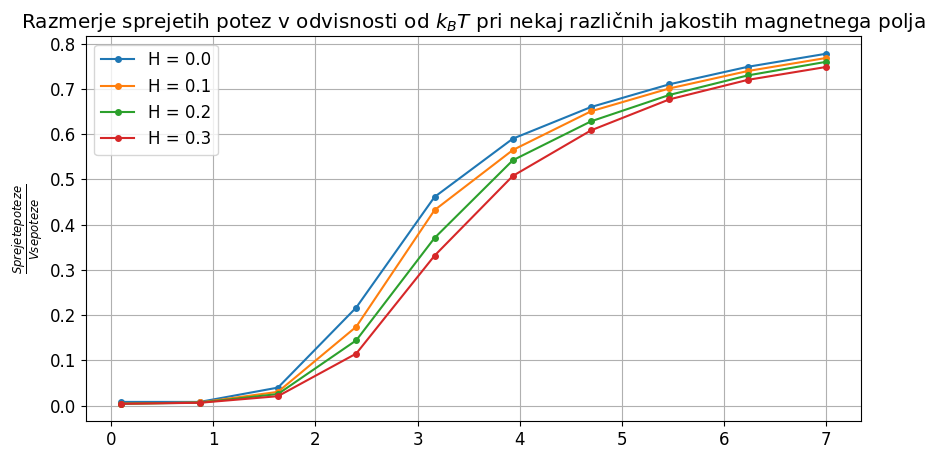
\includegraphics[width=\linewidth]{ising7.png}
\caption{razmerje sprejetih potez v odvisnosti od $k_BT$ pri nekaj različnih vrednostih jakosti magnetnega polje $H$.}
\end{figure}

\section{Zaključek}

V nalogi smo se naučili uporabljati Matropolisov algoritem. Aplicirali smo ga na členkasti verižnici ter isingovemu modelu kristala.

\end{document}